\chapter{Arduino Projects}

    \section{Install Visual Micro plug--in}
    
Visual Micro is a plug--in for Microsoft Visual Studio with C++ installed. It allows to create Arduino IDE compatible projects to 
develop embedded software using the power of the Visual Studio IDE. 

To install this plug--in, follow the next steps: 

\begin{enumerate} 
	
	\item Open your release of Visual Studio.
	\item Click on \textit{Tools/Add ext and updates...}.
	\item Select  \textit{Arduino IDE Visual Studio}.
	\item Close Visual Studio. 
	\item Visual Micro plug--in will start to install. 
	\item After Arduino IDE is installed, open Visual Studio.  
	\item Click on  \textit{VICRO/Ide/configure IDE location...} and  specify where your Arduino folder is located. 
	\item Click \textit{OK}.
		
\end{enumerate}



    \section{Create an Arduino Project}

\begin{enumerate} 
	
	\item Open your release of Visual Studio.
	\item Click on \textit{File/New/Project...} (Figure \ref{fig:Pro1}).
	\item In the \textit{Visual C++} menu select \textit{Arduino Project}.
	\item Change \textit{Name} (project name) to ``HelloWorld''. 
	\item Change the \textit{Location} of the solution to \textit{/Desktop}.
	\item Change the \textit{Solution name} to ``ArduinoProjects''.  
	\item Select option \textit{Create directory for solution}.
	\item Click \textit{OK}.		
\end{enumerate}

Visual Studio will create a folder in the Desktop with the name ``ArduinoProjects'' to hold the complete solution. Inside this folder another folder named ``HelloWorld'' will contain the project \texttt{HelloWorld.ino}. In this case this project contains only one file. In order to be compatible with the Arduino IDE this folder and the Arduino \texttt{.ino} file should have the same name. 

\vspace{0.5cm}
    \section{Execute the ``Hello world'' with Arduino}

Now it is a good practice to determine if the Arduino compiler is properly installed. To verify the installation, we need an Arduino board and we will proceed with the following steps: 

\begin{enumerate} 
	
	\item Download the latest version of the Arduino IDE and unzip its content to same folder. 
	\item Open the visual studio solution that we have created in the last section.
	\item Select the location of the Arduino IDE from the VMICRO tab of the Visual Studio window. 
	\item Select the specific Arduino board that we have.
	\item Plug the Arduino board with a USB wire. 
	\item Select the Serial port in which the Arduino board is discovered: COM1, COM2, ...
	\item Copy and paste the following code in the \texttt{HelloWorld.ino} file:  \vskip \baselineskip 
	
	\lstinputlisting[language=C, firstline=1, lastline=27]{Listing/Helloworld.cpp}

	\item Click on \textit{VMICRO/Build and Upload}.
	\item After the output windows shows: ``The upload process has finished'', click on the serial monitor for the selected port (Figure \ref{fig:arduino}). It will open a serial COM17 window showing the results of the program. Every 5 seconds, the message : ``Hello World'' will appear on the serial terminal.
    
	\begin{figure}[h]
		\centering
		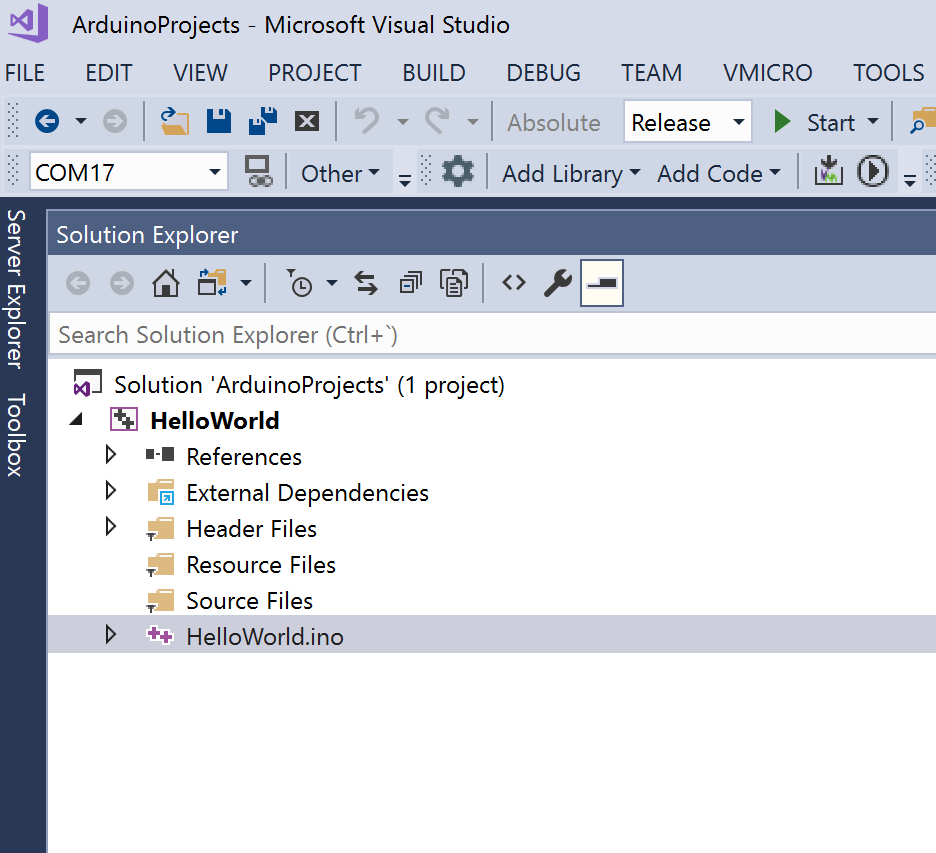
\includegraphics[width= 10cm]{Figures/Arduino.png}
		\caption{Icon to open the Serial monitor close to the selected port: COM17}
		\label{fig:arduino}
	\end{figure}
 
\end{enumerate}


\begin{IN}
    More project/solution examples with Arduino can be downloaded from \url{https://github.com/jahrWork/Visual-Studio-projects}.
\end{IN}

    \section{Configuring complex projects}
    
Visual Studio is useful when we  are dealing with very complex projects in which many libraries of different codes files are involved. 
	
Besides of the internal libraries of the Arduino IDE, Visual Studio can share external libraries with the Arduino project as any other programming language. 
To specifically configure some project, we propose to start from a simple project to increase gradually the complexity by adding different external libraries. 	

To do that, we will start from a new project named: \textit{Automation}. This project is going to blink a led by using an external file or shared item named: \textit{Leds}. 

\newpage
\begin{enumerate} 
	\item Open the visual studio solution that we have created: \textit{ArduinoProjects}. 
	\item Add a new Arduino project to the same solution named: \textit{Automation} as we did to create ``HelloWorld''.  
	\item Add a new share item:
	 \textit{File/New/Project/Add/Visual C++/Arduino Shared Code Project}.
	\item Select \textit{Add to solution}.
	\item Name \textit{Leds} the new project. 
	\item Create two files: \texttt{LedClass.h} and \texttt{LedClass.cpp} inside this share item. 
	\item Copy and paste the following code in the \texttt{Ledclass.h} file: 
	
    %\newpage
	\lstinputlisting[language=C, firstline=2, lastline=27]{Listing/LedClass.h}
	
    %\newpage
	\item Copy and paste the following code in the  \texttt{Ledclass.cpp} file: 
	
	\lstinputlisting[language=C, firstline=2, lastline=27]{Listing/Ledclass.cpp}
	
	\item Right click on \textit{References} of the project \textit{Automation}, then click on \textit{Add references} and select \textit{Leds}.
	
    \item Click on \textit{VMICRO/Build and Upload}.
\end{enumerate} 

	
%\section{Arduino FAQ}


    \FloatBarrier
    \section{Installing C++ Compiler}

If you have installed Visual Studio following this guide you do not have to install anything else since the C++ compiler was included in the first steps. 

In case you do not have the necessary tools already included in the IDE open the Visual Studio Installer as an administrator and click on \textit{Modify}. We have to select in the \textit{Workloads} (in the tab reserved for Windows) the default tools related to ``Development for Desktop with C++'' (see Figure \ref{fig:Instalacion1}). We click on \textit{Modify} and wait for the process to finish the download and installation. 



    \FloatBarrier
    \section{Create a C++ project}

To create a C++ project, proceed with the following steps: 

\begin{enumerate}
    \item Open Visual Studio.
    \item Click on \textit{File/New/Project...} (Figure \ref{fig:Pro1}).
    \item Deploy the field \textit{Language} and select \textit{C++}, then click on \textit{Empty Project} (see Figure \ref{fig:C++1}).
    \item Change the \textit{Project Name}, for example ``HelloWorld'' in this case (see Figure \ref{fig:C++2}). 
    \item Change the \textit{Location} of the solution.
    \item Change the \textit{Solution name} to ``C++Projects''.  
    \item Click on \textit{Create}.
\end{enumerate}

\begin{figure}
    \centering
    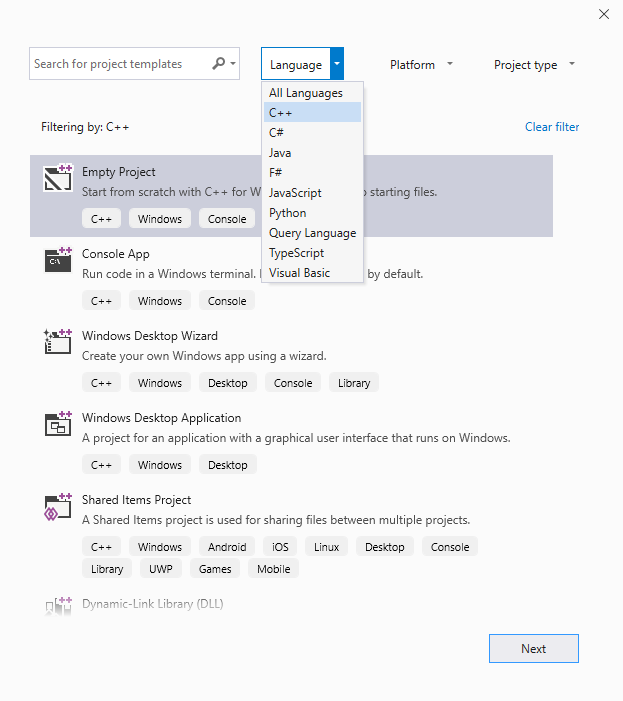
\includegraphics[width= \textwidth]{Figures/C++1}
    \caption{Window for creating a project in Visual Studio 2019 Community version. We have filtered by C++ and chosen Empty Project.}
    \label{fig:C++1}
\end{figure}

\begin{figure}
    \centering
    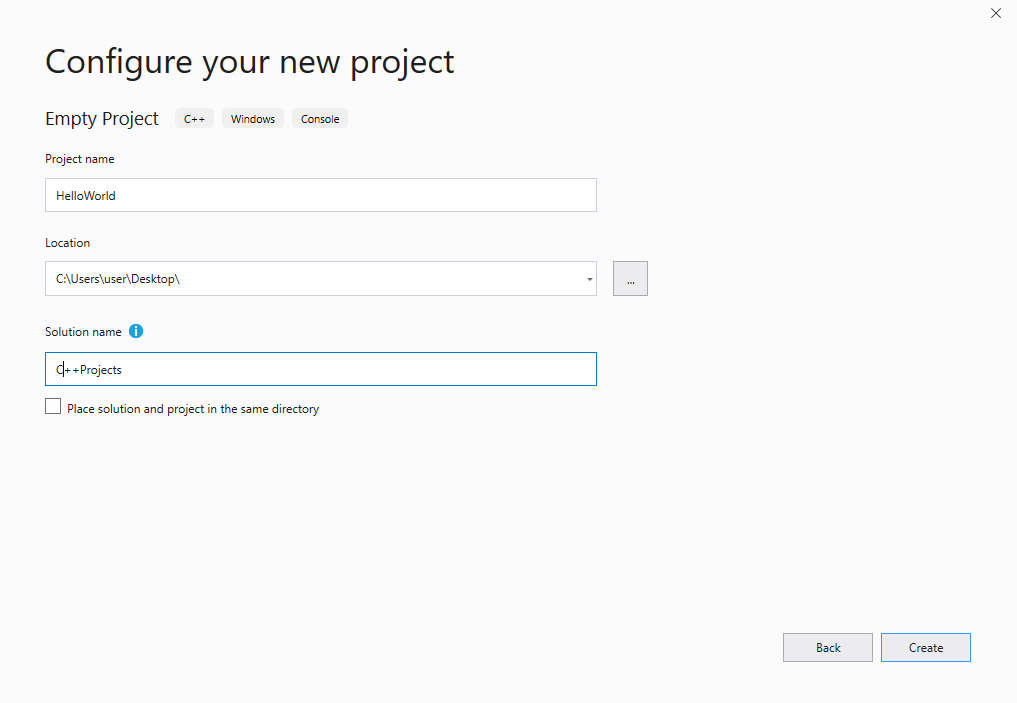
\includegraphics[width= \textwidth]{Figures/C++2}
    \caption{In this window we can create a new Project, a new Solution and specify the names for both and the location for the folders.}
    \label{fig:C++2}
\end{figure}

    
    
    \FloatBarrier
    \section{Execute the ``Hello world'' example with C++}
    
Now we are going to execute our first example in C++, the Hello World program. Firstly, include a new source file to the project by clicking with the right button in the folder ``Source Files'' and on \textit{Add/New Item...} (see Figure \ref{fig:C++3}). Secondly, choose \textit{C++ File (.cpp)} in the tab \textit{Installed/Visual C++}, change the name of the file to \texttt{HelloWorld.cpp} and click on \textit{Add} (Figure \ref{fig:C++4}). You will find a blank file where copying the following code: \vskip \baselineskip 

\begin{lstlisting}[language=C++, caption={Hello World example in C++.}, label={lst:C++example}]
#include <iostream>
using namespace std;

int main() 
{
    cout << "Hello, World!";
    return 0;
}
\end{lstlisting}

To compile, link and execute the program follow the next steps (the box in Figure \ref{fig:C++5} shows the icons for building and executing the project):

\begin{enumerate}
    \item Click on \textit{BUILD/Build solution} or click on the corresponding icon. The program is compiled and linked (Figure \ref{fig:C++5}). 
    \item Click on \textit{DEBUG/Start Without Debugging} or click the corresponding icon. The program is executed. 
\end{enumerate}
 
\begin{IN}
    More project/solution examples with C++ language can be downloaded from: 
    
     \url{https://github.com/jahrWork/Visual-Studio-projects}.
\end{IN}


\begin{figure}
    \centering
    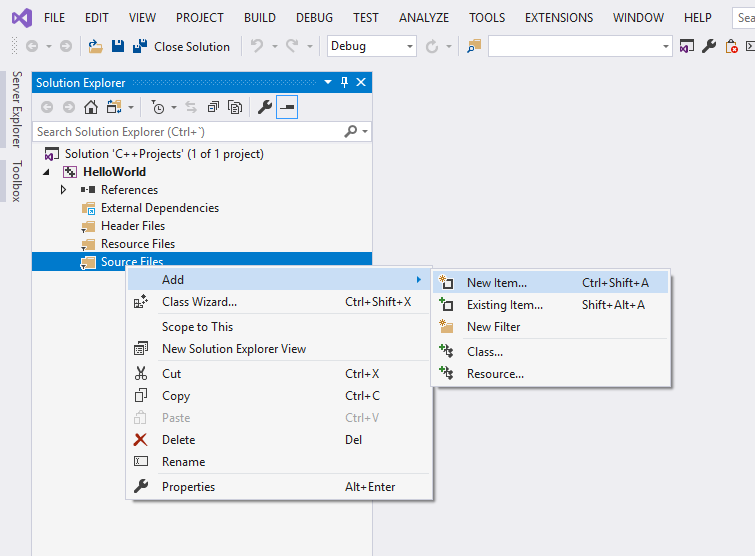
\includegraphics[width= \textwidth]{Figures/C++3}
    \caption{Menu where adding new or existing files to our project.}
    \label{fig:C++3}
\end{figure}

\begin{figure}
    \centering
    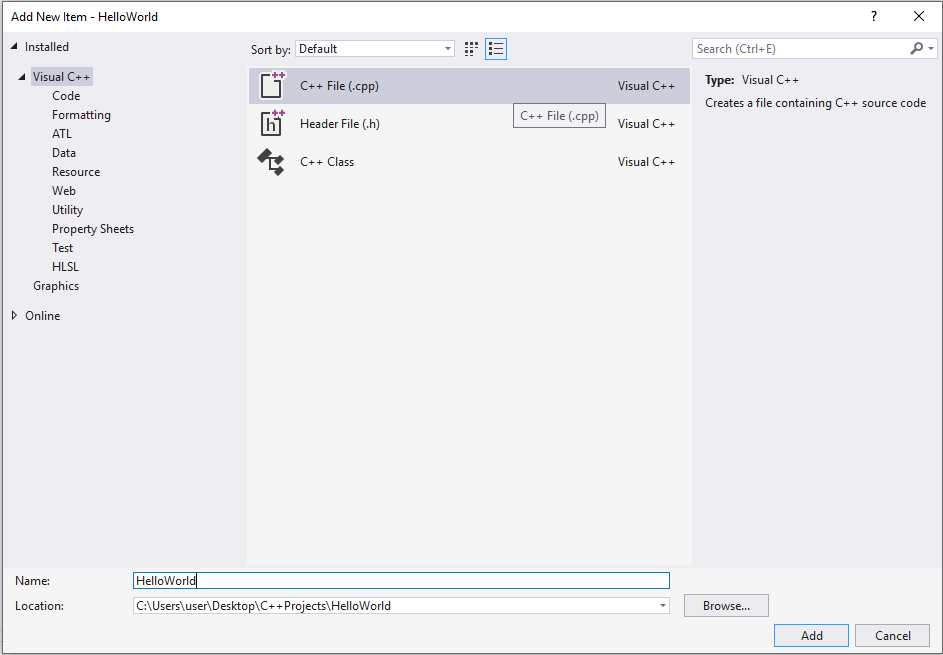
\includegraphics[width= \textwidth]{Figures/C++4}
    \caption{Window where choosing the C++ File. Name it ``HelloWorld'' and add it to the project. The \texttt{.cpp} file stores the source code for a C++ program.}
    \label{fig:C++4}
\end{figure}    
 
\begin{figure}
    \centering
    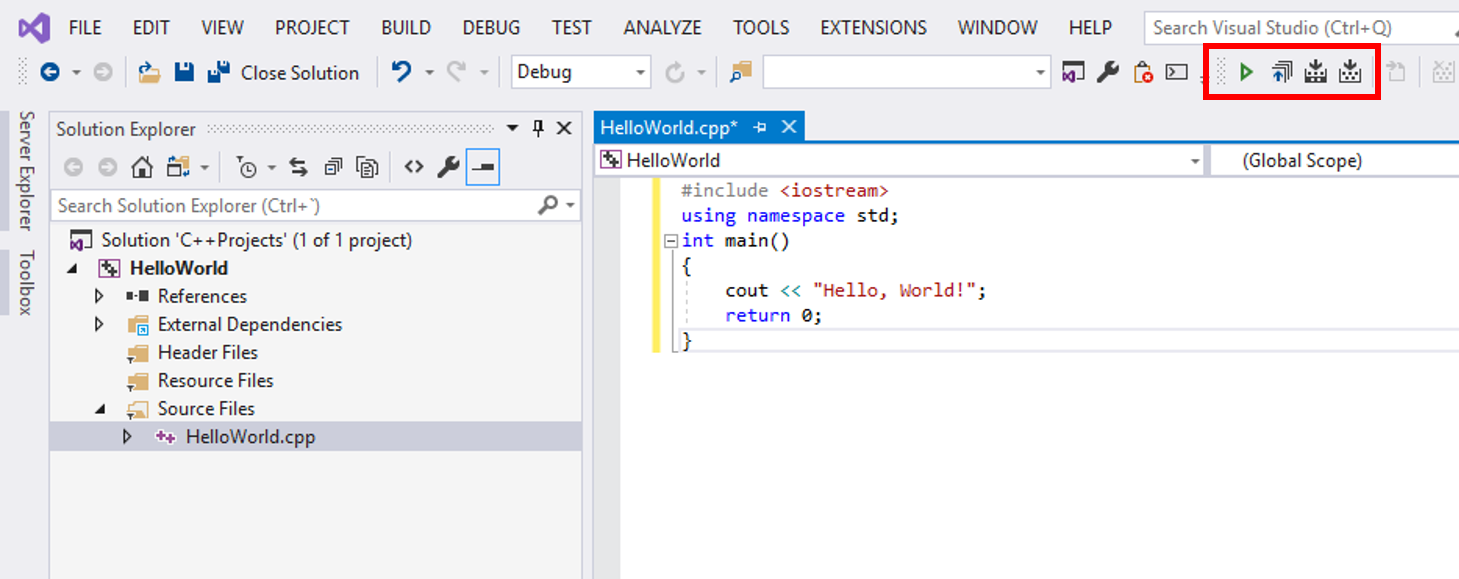
\includegraphics[width= \textwidth]{Figures/C++5}
    \caption{Final aspect of the project, click on \textit{Build the project} and execute it without debugging to see the result.}
    \label{fig:C++5}
\end{figure}    
 
